\documentclass[12pt,a4paper]{article}

\usepackage[top=2.45cm,bottom=2.15cm,left=2.65cm,right=2.65cm,headheight=18pt,headsep=0.55cm]{geometry}
\usepackage{fontspec}
\usepackage{xeCJK}
\usepackage{graphicx}
\usepackage{array}
\usepackage{xcolor}
\usepackage{fancyhdr}
\usepackage{setspace}
\usepackage{indentfirst}
\usepackage{hyperref}
\usepackage{amsmath}
\usepackage{amssymb}
\usepackage{multirow}
\usepackage{diagbox}
\usepackage{booktabs}
\usepackage{tikz}
\usepackage{tocloft}

\newcommand{\SongtiName}{Songti SC}
\IfFontExistsTF{Songti SC}{\renewcommand{\SongtiName}{Songti SC}}{%
  \IfFontExistsTF{STSong}{\renewcommand{\SongtiName}{STSong}}{%
    \IfFontExistsTF{SimSun}{\renewcommand{\SongtiName}{SimSun}}{\renewcommand{\SongtiName}{Noto Serif CJK SC}}}}

\setmainfont{\SongtiName}
\setCJKmainfont[AutoFakeBold=2.4]{\SongtiName}
\setCJKsansfont[AutoFakeBold=2.4]{\SongtiName}
\IfFontExistsTF{Menlo}{\setmonofont{Menlo}[Scale=MatchLowercase]}{\setmonofont{Latin Modern Mono}[Scale=MatchLowercase]}
\XeTeXlinebreaklocale "zh"
\XeTeXlinebreakskip = 0pt plus 1pt
\hypersetup{hidelinks}

\definecolor{lightgray}{RGB}{218,218,218}

\pagestyle{fancy}
\fancyhf{}
\fancyhead[L]{\fontsize{10.5pt}{13pt}\selectfont 重庆理工大学}
\fancyhead[R]{\fontsize{10.5pt}{13pt}\selectfont 《数据结构》实验案例}
\renewcommand{\headrulewidth}{0.55pt}
\fancyfoot[C]{\fontsize{10.5pt}{13pt}\selectfont\thepage}

\setlength{\parindent}{2em}
\setlength{\parskip}{0pt}
\renewcommand{\baselinestretch}{1.0}
\setcounter{tocdepth}{2}
\renewcommand{\contentsname}{目录}
\renewcommand{\cftsecleader}{\cftdotfill{\cftdotsep}}
\renewcommand{\cftsubsecleader}{\cftdotfill{\cftdotsep}}
\setlength{\cftsecindent}{0pt}
\setlength{\cftsubsecindent}{1.35cm}
\setlength{\cftsecnumwidth}{0pt}
\setlength{\cftsubsecnumwidth}{0pt}
\setlength{\cftbeforesecskip}{0.1cm}
\setlength{\cftbeforesubsecskip}{-0.1cm}
\renewcommand{\cftsecfont}{\fontsize{10.5pt}{12pt}\selectfont\bfseries}
\renewcommand{\cftsecpagefont}{\fontsize{10.5pt}{12pt}\selectfont\bfseries}
\renewcommand{\cftsubsecfont}{\fontsize{9.5pt}{10pt}\selectfont}
\renewcommand{\cftsubsecpagefont}{\fontsize{9.5pt}{10pt}\selectfont}

\newcommand{\blankline}{\rule{2.45cm}{0.4pt}}
\newcommand{\expchapter}[1]{%
  \phantomsection\addcontentsline{toc}{section}{#1}%
  \begin{center}{\fontsize{16pt}{24pt}\selectfont\bfseries #1}\end{center}}
\newcommand{\sect}[1]{%
  \phantomsection\addcontentsline{toc}{subsection}{【#1】}%
  \vspace{0.15cm}\noindent{\bfseries【#1】}\par}
\newcommand{\figcaption}[1]{%
  \begin{center}{\fontsize{9.5pt}{12pt}\selectfont #1}\end{center}}
\makeatletter
\newcommand{\makerealtoc}{%
  \thispagestyle{fancy}%
  \vspace*{-0.9cm}%
  \begin{center}
    {\fontsize{18pt}{28pt}\selectfont\bfseries 目录}
  \end{center}
  \vspace{0.15cm}
  \@starttoc{toc}
}
\makeatother

\begin{document}
\fontsize{10.5pt}{15.8pt}\selectfont

\begin{titlepage}
\thispagestyle{fancy}
\centering
\vspace*{3.05cm}
{\fontsize{46pt}{58pt}\selectfont\bfseries 数据结构\par}
\vspace{3.15cm}
{\fontsize{34pt}{46pt}\selectfont\bfseries 实验案例\par}
\vspace{3.45cm}
{\fontsize{18pt}{28pt}\selectfont\bfseries 主讲老师：卢玲\par}
\vfill
{\fontsize{18pt}{28pt}\selectfont\bfseries 计算机科学与技术专业\par}
\vspace{0.25cm}
{\fontsize{18pt}{28pt}\selectfont\bfseries 二〇二二年四月\par}
\vspace{1.9cm}
\end{titlepage}

\setcounter{page}{2}
\clearpage
\makerealtoc

\clearpage
\expchapter{实验一\quad 计算两篇文章的相似度}
\sect{教学目标}
\noindent\hspace*{2em}知识和能力目标：熟练掌握和应用线性表解决实际问题。价值目标：\par
\noindent\hspace*{2em}科学精神：论文抄袭是一种非常严重的学术不端行为，我们不仅需要尊重他人的知识产权，同时也需要保护自己的知识产权，对自己的论文、报告、代码等各种学习成果加以保护。\par
\noindent\hspace*{2em}人文素质：你在日常学习中如何保护自己的知识产权？你在日常学习中有哪些尊重他人知识产权的做法？\par
\sect{问题描述}
\noindent\hspace*{2em}文本相似度计算在信息检索、数据挖掘、机器翻译、文档复制检测等领域有着广泛的应用。例如网络舆情监控问题。假设你开发了一个微博网站，并且已经把世界上骂人的句子都收录进了数据库，那么当一个用户发微博时，最简单的办法就是将用户的微博文本与骂人句子数据库进行比较，s判断其相似性，如果达到某种相似度，则用户的微博就不允许发出。\par
\noindent\hspace*{2em}本问题的任务是：编写程序，计算任意两篇文章的相似度。假设如下：\par
\noindent\hspace*{2em}文章是英文文章，每个单词之间有空格分隔。\par
\noindent\hspace*{2em}文章长度不限，其中包含的英文单词数未知。\par
\noindent\hspace*{2em}提供 3 种长度文章的测试结果：20 词左右，300 词左右，300 词以上\par
\sect{基本思路}
\noindent\hspace*{2em}判断文章相似度的策略很多，本任务请采用余弦相似度算法进行计算，具体描述如下。\par
\noindent\hspace*{2em}一般来说，如果两篇文章的用词越相似，可以大致认为它们的内容越相似。对任意文本 A\textbackslash{}B，我们可以用余弦相似度来计算其相似度。具体描述如下。\par
\noindent\hspace*{2em}文本 \textbf{A}： 我喜欢看电视，不喜欢看电影\par
\noindent\hspace*{2em}文本 \textbf{B}： 我不喜欢看电影，也不喜欢看电视可以从词频入手计算文本 A 和 B 的相似度。\par
\noindent\textbf{文本A 和 B 中包含如下词：}\par
\noindent\hspace*{2em}文本 \textbf{A}：我 喜欢 看 电视 ， 不 喜欢 看 电影 。\par
\noindent\hspace*{2em}文本 \textbf{B}：我 不 喜欢 看 电视 ， 也 不 喜欢 看 电影 。首先合并所有词：\par
\noindent\hspace*{2em}我 喜欢 看 电视 电影 不 也然后计算每一篇文本的词频：\par
\noindent\hspace*{2em}由此得到每一篇文章的词频向量\par
\noindent\hspace*{2em}我们可以把这两个向量想象成 \textbf{7}\textbf{ }维空间中的两条线段\footnote{当然也可以把两篇文章看成是 7 维空间中的两个点。}，它们分别从原点（[0, 0, ...]）出发，指向\par
\noindent\hspace*{2em}不同方向。两条线段之间形成一个夹角，如果夹角为 0 度，意味着方向相同、线段重合；如果夹角\par
\noindent\hspace*{2em}为 90 度，意味着形成直角，方向完全不相似；如果夹角为 180 度，意味着方向正好相反。因此，我们可以通过夹角的大小，来判断向量的相似程度。夹角越小，就代表越相似。\par
\begin{center}
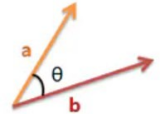
\includegraphics[width=0.28\textwidth]{images/exp1-1.png}
\end{center}
\noindent\hspace*{2em}假定 a 向量是[x1, y1]，b 向量是[x2, y2]，那么可将余弦定理改写成下面的形式：\par
\begin{equation*}
\cos\theta = \frac{x_{1}x_{2}+y_{1}y_{2}}{\sqrt{x_{1}^{2}+y_{1}^{2}}\,\times\,\sqrt{x_{2}^{2}+y_{2}^{2}}}
\end{equation*}
\noindent\hspace*{2em}余弦的这种计算方法对 n 维向量也成立。假定A 和B 是两个n 维向量，\par
\noindent\hspace*{2em}A 是 [A1, A2, ..., An] ，B 是 [B1, B2, ..., Bn] ，则 A 与 B 的夹角 θ 的余弦等于：\par
\begin{equation*}
\begin{aligned}
\cos\theta &= \frac{\sum\limits_{i=1}^{n}(A_{i}\times B_{i})}{\sqrt{\sum\limits_{i=1}^{n}(A_{i})^{2}}\,\times\,\sqrt{\sum\limits_{i=1}^{n}(B_{i})^{2}}} \\
&= \frac{A\cdot B}{|A|\times|B|}
\end{aligned}
\end{equation*}
\noindent\hspace*{2em}使用这个公式，我们就可以计算得到文本A 与文本 B 的余弦相似度如下：\par
\begin{equation*}
\begin{aligned}
\cos\theta &= \frac{1\times 1+2\times 2+2\times 2+1\times 1+1\times 1+1\times 2+0\times 1}{\sqrt{1^{2}+2^{2}+2^{2}+1^{2}+1^{2}+1^{2}+0^{2}}\,\times\,\sqrt{1^{2}+2^{2}+2^{2}+1^{2}+1^{2}+2^{2}+1^{2}}} \\
&= \frac{13}{\sqrt{12}\times\sqrt{16}} \\
&\approx 0.938
\end{aligned}
\end{equation*}
\sect{实验结果及分析}
\noindent\hspace*{2em}1. 实验结果（课程目标 3：2）\par
\noindent\hspace*{2em}请描述实验过程，包括编程环境、测试数据等，用图、表等方式，呈现实验结果。\par
\noindent\hspace*{2em}（1）实验过程描述\par
\noindent\hspace*{2em}1. 本实验用XX 语言开发，编译环境为 XX，运行机器为本人笔记本电脑或 XXXX。由X 人                         设计方案，本人独立完成编码和测试。\par
\noindent\hspace*{2em}2. 测试数据选取思路为：典型，XXX，XXX。累计选取X 组数据进行测试。\par
\noindent\hspace*{2em}3. XXX 部分的逻辑是测试重点。因为 XXX\par
\noindent\hspace*{2em}（2）测试结果\par
\noindent\hspace*{2em}用图、表等方式，呈现实验结果。\par
\noindent\hspace*{2em}2. 结果及方案分析（课程目标 1：2）\par
\noindent\hspace*{2em}（1）本实验的重点及难点\par
\noindent\hspace*{2em}本实验设计的重点为 XXXX。\par
\noindent\hspace*{2em}本实验设计的难点为 XXXX。\par
\noindent\hspace*{2em}（2）本实验设计的优点及可以改进的方向\par
\noindent\hspace*{2em}实验完全或部分实现了预计功能。          设计得较为充分之处为XX\par
\noindent\hspace*{2em}设计的可优化处包括：XXXX\par
\noindent\hspace*{2em}3. 还有那些相似度计算方法？谈谈你的个人观点。（思政目标）\par
\noindent\hspace*{2em}4. 附件：源程序代码\par
\noindent\hspace*{2em}源代码复制粘贴在这里（六号字，分栏，单倍行距不要对齐网格）\par
\clearpage
\expchapter{实验二\quad 中国地图四染色问题}
\sect{教学目标}
\noindent\hspace*{2em}知识和能力目标：熟练掌握和应用栈结构解决实际问题，本例主要是从递归算法到非递归算法的问题。\par
\noindent\hspace*{2em}价值目标：\par
\noindent\hspace*{2em}科学精神：希望你了解四色定理的产生及研究历程，理解科学研究的严谨性，、长期性及其对人类社会发展的深远影响。\par
\noindent\hspace*{2em}人文素质：你是否知道什么是飞地？\par
\sect{问题描述}
\noindent\hspace*{2em}四色问题又称四色猜想、四色定理，是世界近代三大数学难题之一。1852 年毕业于伦敦大学的佛朗西斯·格斯里（Francis Guthrie）在一家科研单位进行地图着色工作时，发现了一个有趣现象：每幅地图都可以只用四种颜色着色，就能使有共同边界的国家都着上不同颜色（不含飞地\footnote{飞地，是一种特殊的人文地理现象，指隶属于某一行政区管辖但不与本区毗连的土地。}）。那么，这是一个因地图不够复杂的巧合？还是一个确认的定理呢？\par
\noindent\hspace*{2em}多年以来，数学家们为证明四色定理绞尽脑汁，所引进的概念与方法刺激了拓扑学与图论的发展。在四色问题研究中，不少新的数学理论和数学计算技巧随之产生，例如将地图的着色问题转化为图论问题，丰富了图论的内容。不仅如此，“四色问题”在有效设计航空班机日程表、设计计算机的编码程序上都起到了推动作用。\par
\noindent\hspace*{2em}中华人民共和国有 34 个省级行政区，含 23 个省、5 个自治区、4 个直辖市、2 个特别行政区\footnote{中国行政区划（2020 年）. 行政区划网．}。\par
\begin{center}
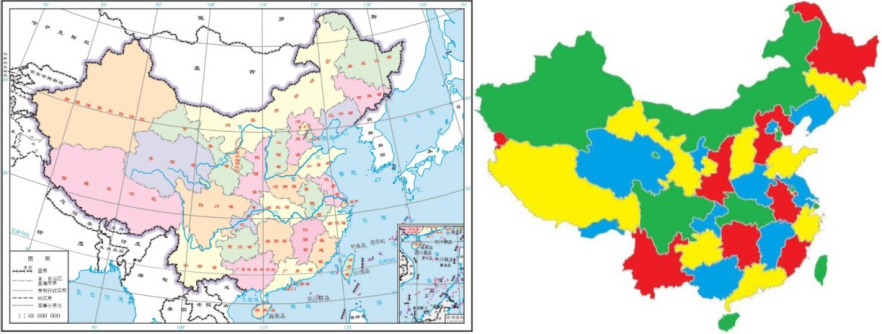
\includegraphics[width=0.85\textwidth]{images/exp2-1.png}
\end{center}\par

\noindent\hspace*{2em}\textbf{23}\textbf{ }个省分别为：河北省、山西省、辽宁省、吉林省、黑龙江省、江苏省、浙江省、安徽省、福建省、江西省、山东省、河南省、湖北省、湖南省、广东省、海南省、四川省、贵州省、云南省、陕西省、甘肃省、青海省、台湾省。\par
\noindent\hspace*{2em}\textbf{5 }个自治区分别为：内蒙古自治区、广西壮族自治区、西藏自治区、宁夏回族自治区、新疆维吾尔自治区。\par
\noindent\hspace*{2em}\textbf{4}\textbf{ }个直辖市分别为：北京市、天津市、上海市、重庆市。\par
\noindent\hspace*{2em}\textbf{2}\textbf{ }个特别行政区分别为：香港特别行政区、澳门特别行政区。本问题的任务是：\par
\noindent\hspace*{2em}编写程序，用四种颜色对中国地图染色，输出任意一种染色方案。\par
\noindent\hspace*{2em}是否能用 \textbf{3}\textbf{ }种颜色对中国地图染色？请编程验证。假设如下：\par
\noindent\textbf{四种颜色不限，输出形式不限}\par
\noindent\textbf{用递归和非递归两种算法来实现}\par
\sect{基本思路}
\noindent\textbf{地图可用图的邻接矩阵方法来存储}\par
\noindent\hspace*{2em}染色过程可借助一个栈结构，由于省级行政区数已知为 34，因此可使用顺序栈。\par
\noindent\hspace*{2em}以下是一个含 7 个地区的地图四染色结果。\par
\begin{center}
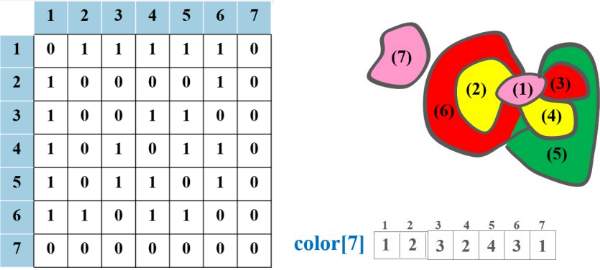
\includegraphics[width=0.55\textwidth]{images/exp2-2.png}
\end{center}
\noindent\textbf{染色时不妨总是从 1 号色开始试探}\par

\sect{实验结果}
\noindent\hspace*{2em}1. 实验重点及难点\par
\noindent\hspace*{2em}（1）本实验的重点\par
\noindent\hspace*{2em}（2）本实验的难点\par
\noindent\hspace*{2em}2. 实验结果\par
\noindent\hspace*{2em}请描述实验过程，包括编程环境、测试数据等，用图、表等方式，记录、呈现实验结果。\par
\noindent\hspace*{2em}（1）实验过程描述\par
\noindent\hspace*{2em}（2）测试结果\par
\noindent\hspace*{2em}3. 实验方案分析\par
\noindent\hspace*{2em}（1）本实验设计的优点\par
\noindent\hspace*{2em}（2）本实验设计上的不足\par
\noindent\hspace*{2em}4. 附件：源程序代码\par
\noindent\hspace*{2em}源代码复制粘贴在这里（六号字，分栏，单倍行距不要对齐网格）\par
\clearpage
\expchapter{实验三\quad 操作系统的时间片轮转调度算法}
\sect{教学目标}
\noindent\hspace*{2em}关键词：队列，分时操作系统，时间片轮转调度算法\par
\noindent\hspace*{2em}知识和能力目标：熟练掌握队列的存储及其操作方法，理解队列适用的问题场景。价值目标：\par
\noindent\hspace*{2em}职业素养（工程与社会）：计算机系统的设计与实施，是一个系统工程，或者说，它就是一个工程问题。工程师在解决问题时，总是需要在资源使用和资源保护方面寻找平衡点。时间片轮转调度算法很有意思，你可能会发现，虽然时间片的大小、进程的执行时间等因素间存在强相关性，但为了获得良好的带权周转时间，却很难有一个标准答案，需要我们权衡多种因素，按需进行设计和选择。作为未来的计算机工程师，你在处理实际问题时，应该对此有充分的认知和心理准备。\par
\noindent\hspace*{2em}人文素质：你认为作为计算机工程师，我们工作中的美学体现在哪些方面？\par
\sect{问题描述}
\noindent\hspace*{2em}操作系统（Operating System，OS）是管理计算机硬件与软件资源的程序，是计算机系统的内核与基石。操作系统需要管理内存、决定系统资源供需的优先次序、控制输入与输出设备、操作网络、管理文件系统等，操作系统也提供一个让用户与系统交互的界面。\par
\noindent\hspace*{2em}分时操作系统（Time-sharing operating System）是指在一台主机上连接了多个带有显示器和键盘等设备的终端，允许多个用户同时通过自己的终端以交互方式共享使用计算机的系统。在分时操作系统管理下，终端用户通过各自的终端向系统发出命令请求，系统采用时间 片轮转法的方式，来接收每个用户的命令并处理服务请求，同时通过交互方式在终端上向用户显示处理的结果。即系统将 CPU 的执行时间分割为一个个时间段（称为时间片），然后轮流分配给每个用户使用，每个用户程序每次只能在CPU 上运行一个时间片。由于时间间隔很短，每个用户感觉自己独占了计算机。Unix和 Linux 是典型的分时操作系统。\par
\begin{center}
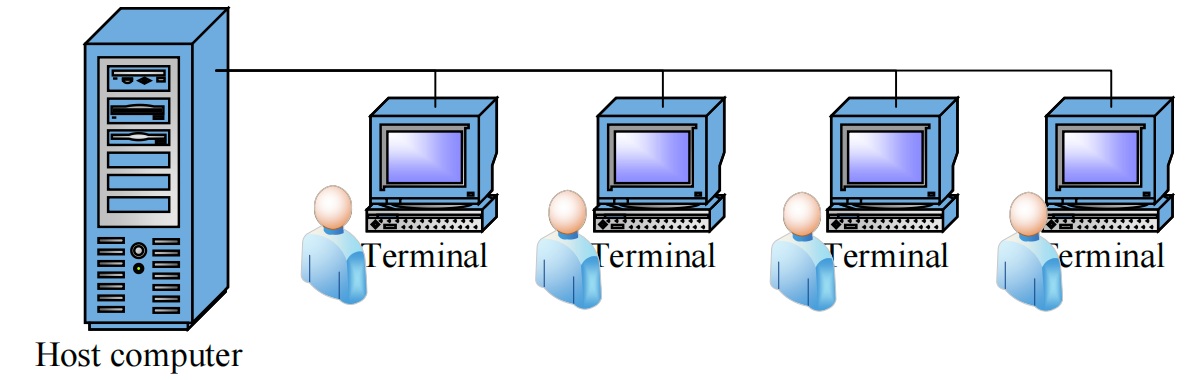
\includegraphics[width=0.65\textwidth]{images/exp3-1.png}
\end{center}
\noindent\hspace*{2em}本问题的任务是：编写程序，模拟实现分时操作系统的时间片轮转调度算法。\par
\sect{基本思路}
\noindent\hspace*{2em}时间片轮转（\textbf{Round Robin}，\textbf{RR}）调度算法：为分时操作系统设计。在期的时间片轮转法中，系统将所有就绪进程按先来先服务的原则排成一个队列。每次调度时，把CPU 分配给队首进程，并令其执行一个时间片。时间片\footnote{在时间片轮转算法中，时间片的大小对系统性能有很大影响。很小的时间片有利于短作业，因为它能较快地切换，但会频繁地发生中断、进程切换，从而增加系统开销。如时间片太长，使每个进程都能在一个时间片内完成，时间片轮转算法便退化为 FCFS 算法，无法满足交互式用户的需求。}的大小从几 \textit{ms}\textit{ }到几百 \textit{ms}。当执行的时间片用完时，由一个计时器发出时钟中断，调度程序据此信号来停止该进程，并将它送往就绪队列的末尾；然后再把处理机分配给就绪队列中新的队首进程，也让它执行一个时间片。如此反复，就可以保证就绪队列中的所有进程在一个给定的时间段内均能获得若干时间片的处理机执行时间。也即，操作系统能在给定时间段内响应所有用户的请求。\par
\noindent\textbf{\textbf{RR}\textbf{ }算法思路：}\par
\noindent Step1：将需要运行的进程依次放入就绪队列 Q\par
\noindent Step2：如果 Q 为空，则 return ;否则，从 Q 出队一个进程，让其运行一个时间片的时间。如进程在一个时间未执行完，则其去Q 末尾重新排队，等待下一次调度。\par
\noindent Step3：转 Step2\par
\noindent\hspace*{2em}【例】进程 \textit{\textbf{A}}、\textit{\textbf{B}}、\textit{\textbf{C}}、\textit{\textbf{D}}\textit{\textbf{ }}需运行的时间分别为 20\textit{ms}、10 \textit{ms}、15 \textit{ms}、5 \textit{ms}，均在 0 时刻到达。到达次序为 \textit{\textbf{A}}、\textit{\textbf{B}}、\textit{\textbf{C}}、\textit{\textbf{D}}。如果时间片分别为 1 \textit{ms}\textit{ }和 5\textit{ms}，计算各进程的带权周转时间和平均带权周转时间。分析：根据 \textit{\textbf{RR }}算法，图 4.1 表示了进程执行情况。\par
\begin{figure}[h]
\centering
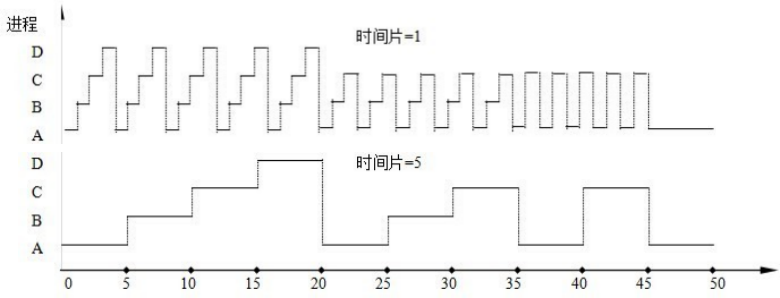
\includegraphics[width=0.95\textwidth]{images/exp3-2.png}
\end{figure}

\noindent\hspace*{2em}进程 \textit{\textbf{i}} 的带权周转时间：$w_i = \dfrac{T_i}{R_i}$，其中 $T_i$ 为周转时间，$R_i$ 为实际运行时间。\par
\noindent\hspace*{2em}所有进程的平均带权周转时间：$W = \left(\sum\limits_{i=1}^{n} w_i\right) \times \dfrac{1}{n} = \left(\sum\limits_{i=1}^{n} \dfrac{T_i}{R_i}\right) \times \dfrac{1}{n}$\par
\noindent\hspace*{2em}\textit{\textbf{RR}} 算法的性能指标如下（以下除带权周转时间外，其余时间单位均为 \textit{ms}）：\par
\begin{center}
\fontsize{8.5pt}{11pt}\selectfont
\renewcommand{\arraystretch}{1.18}
\begin{tabular}{|c|c|c|c|c|c|c|c|}
\hline
到达时间 & 进程名 & 到达时间 & 运行时间 & 开始时间 & 完成时间 & 周转时间 & 带权周转时间 \\ \hline
\multirow{5}{*}{时间片=5} & A & 0 & 20 & 0  & 50 & 50 & 2.5 \\ \cline{2-8}
                       & B & 0 & 10 & 5  & 30 & 30 & 3.0 \\ \cline{2-8}
                       & C & 0 & 15 & 10 & 45 & 45 & 3.0 \\ \cline{2-8}
                       & D & 0 & 5  & 15 & 20 & 20 & 4.0 \\ \cline{2-8}
                       & \multicolumn{5}{c|}{平均周转时间=36.25\quad 平均带权周转时间=3.125} & \multicolumn{2}{c|}{} \\ \hline
\multirow{5}{*}{时间片=1} & A & 0 & 20 & 0 & 50 & 50 & 2.5 \\ \cline{2-8}
                       & B & 0 & 10 & 1 & 34 & 34 & 3.4 \\ \cline{2-8}
                       & C & 0 & 15 & 2 & 45 & 45 & 3.0 \\ \cline{2-8}
                       & D & 0 & 5  & 3 & 20 & 20 & 4.0 \\ \cline{2-8}
                       & \multicolumn{5}{c|}{平均周转时间=37.25\quad 平均带权周转时间=3.225} & \multicolumn{2}{c|}{} \\ \hline
\end{tabular}
\end{center}
\sect{实验结果}
\noindent\hspace*{2em}1. 算法概述：简述算法框架\par
\noindent\hspace*{2em}2. 实验重点或难点\par
\noindent\hspace*{2em}（1）\par
\noindent\hspace*{2em}（2）\par
\noindent\hspace*{2em}3. 实验结果\par
\noindent\hspace*{2em}（1）实验测试描述，及运行结果记录\par
\noindent\hspace*{2em}4. 实验方案分析\par
\noindent\hspace*{2em}（1）本实验设计的优点，不足，时空开销等问题分析\par
\noindent\hspace*{2em}5. 附件：源程序代码\par
\noindent\hspace*{2em}源代码复制粘贴在这里（六号字，分栏，单倍行距不要对齐网格）\par
\clearpage
\expchapter{实验四\quad 翻转的花朵}
\sect{教学目标}
\noindent\hspace*{2em}关键词：数组\par
\noindent\hspace*{2em}知识和能力目标：理解和熟练掌握多维数组的存储及其操作方法，本例主要是对 BMP 位图文件的像素矩阵进行操作。\par
\noindent\hspace*{2em}价值目标：\par
\noindent\hspace*{2em}科学精神：一幅图像，一篇文章，一个社交关系网络，都可以抽象为一个关系矩阵。由此，我们可以将翻转图像、计算文章相似度找到社交网络中的大 V，统一为对矩阵的计算问题。\par
\noindent\textbf{工程观：}\par
\noindent\hspace*{2em}如果有人说，在我们的生活和工作中，数学无处不在，你会如何回应？\par
\sect{问题描述}
\noindent\hspace*{2em}数字图像数据可以用矩阵来表示，因此可以用矩阵理论和矩阵算法对数字图像进行分析和处理。以灰度图像\footnote{灰度图像是一种具有从黑到白 256 级灰度色域或等级的单色图像。该图像中的每个像素用 8 位数据表示，因此像素点值介于黑白间的 256 种灰度中的一种。该图像只有灰度等级，而没有颜色的变化。}为例（图 1）。灰度图像的像素数据就是一个矩阵，矩阵的行对应图像的高（单位为像素），矩阵的列对应图像的宽，矩阵元素对应图像的像素，矩阵元素的值就是像素的灰度值。\par
\begin{center}
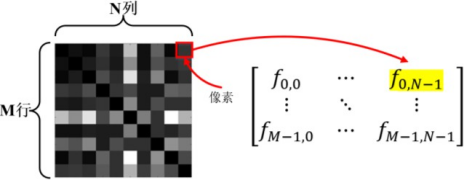
\includegraphics[width=0.5\textwidth]{images/exp4-1.png}
\end{center}
\figcaption{图 1 图像像素矩阵}
\noindent\hspace*{2em}BMP 是一种与硬件设备无关的图像文件格式，采用位映射存储格式。BMP 图像的深度有 1bit（2色）、4bit（16 色）、8bit（256 色）及 24bit（真彩色）。BMP 文件存储位图数据时，图像扫描方式是：在行内按从左到右扫描、在行间从下到上扫描的顺序。Windows 规定图像文件中，一个图像的扫描行所占的字节数必须是 4 的倍数，不足的以 0 填充。\par
\noindent\hspace*{2em}biWidth：图像的宽度，单位是像素\par
\noindent\hspace*{2em}biBitCount：每个像素所需位数，常用 1bit（2 色）、4bit（16 色）、8bit（256 色）、24bit（真彩色）如果 biBitCount = 1，1 个像素 1bit，8 个像素占 1 字节\par
\noindent\hspace*{2em}如果 biBitCount = 4，1 个像素 4bit，2 个像素占 1 字节 如果 biBitCount = 8，1 个像素 8bit，1 个像素占 1 字节如果 biBitCount = 24，1 个像素 24bit，1 个像素占 3 字节\par
\noindent\hspace*{2em}对 BMP 图像，要求是 4 字节对齐，即每行字节数必须为 4 的整数倍，因此满足以 4 字节为对齐单位向下对齐，所以每行字节数为：（8 bit = 1Byte）\par
\noindent\hspace*{2em}PerLineBytes = (((biWidth * biBitCount) / 8 + 3) / 4) * 4\par
\noindent\hspace*{2em}图像的镜像（mirror）分水平镜像和垂直镜像两种，图像的转置可看成是逆时针旋转 90 度。以下是一幅图像的原图、水平镜像、垂直镜像和转置图像。\par
\begin{center}
\begin{minipage}{0.22\textwidth}
\centering
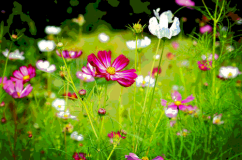
\includegraphics[width=\linewidth]{images/exp4-2.png}
\end{minipage}\hfill
\begin{minipage}{0.22\textwidth}
\centering
\scalebox{-1}[1]{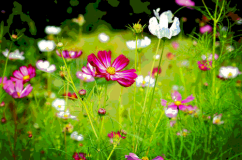
\includegraphics[width=\linewidth]{images/exp4-2.png}}
\end{minipage}\hfill
\begin{minipage}{0.22\textwidth}
\centering
\scalebox{1}[-1]{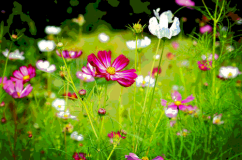
\includegraphics[width=\linewidth]{images/exp4-2.png}}
\end{minipage}\hfill
\begin{minipage}{0.22\textwidth}
\centering
\rotatebox{90}{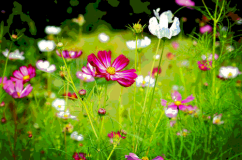
\includegraphics[width=\linewidth]{images/exp4-2.png}}
\end{minipage}
\end{center}

\noindent\hspace*{2em}本问题的任务是：\par
\noindent\hspace*{2em}编写程序，对任意 \textbf{BMP }图像，将其水平镜像、垂直镜像、转置，将处理后的图像保存到文件。假设如下：为简化问题，图像为 256 色BMP 图，也可尝试操作 2 色、16 色BMP 图\par
\sect{基本思路}
\noindent\hspace*{2em}读取BMP 图像：一个 BMP 文件的存储形式如下：\par
\begin{center}
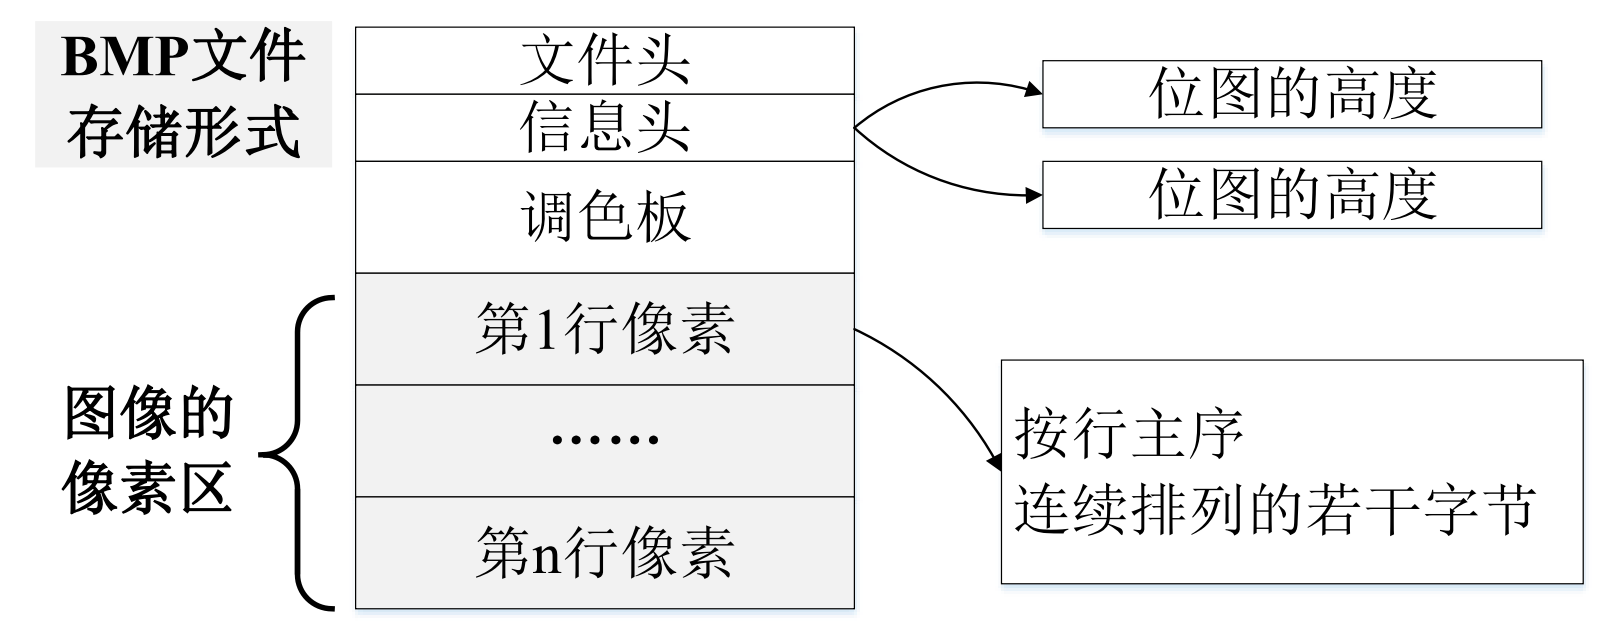
\includegraphics[width=0.85\textwidth]{images/exp4-3.png}
\end{center}

\noindent\hspace*{2em}主要由以下四部分构成\footnote{相关说明：\url{https://blog.csdn.net/aidem\_brown/article/details/80500637}}\footnote{相关说明：\url{https://blog.csdn.net/qq\_36752072/article/details/78151770}}，因此读取一幅 \textbf{256}\textbf{ }色 \textbf{BMP}\textbf{ }图像时，需分别读取以上四部分信息，存 盘也要保存这四部分信息。第 4 部分为我们实际要处理（镜像和转置）的像素数据：位图全部的像素，是按自下向上，自左向右的顺序排列的\footnote{24 位真彩色位图没有颜色表，所以只有 1、2、4 这三部分。}。\par
\begin{center}
\fontsize{8.5pt}{11pt}\selectfont
\renewcommand{\arraystretch}{1.12}
\begin{tabular}{|c|l|p{5cm}|}
\hline
1 & 位图文件头 BITMAPFILEHEADER & BITMAPFILEHEADER：文件头结构 \\ \hline
2 & 位图信息头 BITMAPINFOHEADER & BITMAPINFOHEADER：信息头结构 \\ \hline
3 & 调色板8Palette & RGBQUAD：调色板结构 \\ \hline
4 & 实际的位图数据 ImageDate & unsigned char \\ \hline
\end{tabular}
\end{center}
\noindent\hspace*{2em}图像镜像：设原图宽为 w，高为 h，镜像变换前后，图的宽和高不变。\par
\noindent\hspace*{2em}图像转置：设原图宽为 w，高为 h，转置后图宽为 h，高为w。请自行设计位置计算公式。\par
\sect{实验结果}
\noindent\hspace*{2em}1. 算法概述：简述算法框架\par
\noindent\hspace*{2em}2. 实验重点或难点：\par
\noindent\hspace*{2em}3. 实验结果：实验测试描述，及运行结果记录\par
\noindent\hspace*{2em}4. 实验方案分析：本实验设计的优点，不足，时空开销等问题分析\par
\noindent\hspace*{2em}5. 附件：源程序代码：源代码复制粘贴在这里（六号字，分栏，单倍行距不要对齐网格）\par
\clearpage
\expchapter{实验五\quad 基于 Huffman 编码的文件压缩存储}
\sect{教学目标}
\noindent\hspace*{2em}关键词：哈夫曼编码，数据压缩，哈夫曼树知识和能力目标：\par
\noindent\hspace*{2em}理解和熟练掌握哈夫曼算法，以及哈夫曼编码的方法，本例主要是运用哈夫曼算法对一个文本文件进行压缩操作。\par
\noindent\hspace*{2em}价值目标：\par
\noindent\hspace*{2em}科学精神：希望你了解数据压缩技术的发展历程，通过查阅资料，思考推动各种数据压缩技术发展的动力。\par
\noindent\hspace*{2em}人文素质：你是否了解 mp3、mp4 文件是有损压缩，还是无损压缩？数据压缩的目的是为了什么？作为未来的工程师，如何看待工程与社会的关系？\par
\sect{问题描述}
\noindent\hspace*{2em}现代 IT 产业经常提及“大数据”，据信 2020 年全球信息量将超 40ZB。数据压缩可节省数据存储空间和传输时间。文本、图像、视频、音乐等数据中多有冗余，例如文本中很多字符出现的频率远高于其他字符，图片编码中存在大片的相同区域，电影、声音等类似信号的文件有大量的重复模式。将这些重复区域进行压缩，将大幅减小文件存储空间。\par
\noindent\hspace*{2em}数据压缩的性能指标为压缩时间、压缩率，常分为有损压缩、无损压缩。常说的“无损音乐”就是无损压缩方法。对一串数字 “62389”，现在要把这些数字存进来。有几种方式：\par
\noindent\textbf{int a = 62389;\quad //32 位}\par
\noindent\textbf{short a = 62389;\quad //16 位\footnote{比 short 再小的单位不能存储 52088 了，因为 short 的边界就是 65536-1=65535。char 的边界是 256-1=255}}\par
\noindent\hspace*{2em}将 623 和 89 分开存储，short=623，char=89，16+8=24 位\par
\noindent\hspace*{2em}直接用位输出，623 需 10 位，89 需 7 位，共 17 位\par
\noindent\hspace*{2em}直接用位输出，进一步拆分数据，6，2，3，8，9，分别用位存入，就是 3 位+2 位+1 位+4位+4 位=14 位\par
\noindent\hspace*{2em}最终第五种方式占用空间最小，这是最粗糙的一种数据压缩方式。\par
\noindent\hspace*{2em}假设要传输如下字符串：AEEBBBDDDDDDCCCCCCCC，共 20 个字符，按约定转为二进制数：\par
\begin{center}
\fontsize{8.5pt}{11pt}\selectfont
\renewcommand{\arraystretch}{1.12}
\begin{tabular}{|c|c|c|c|c|}
\hline
A & B & C & D & E \\ \hline
000 & 001 & 010 & 011 & 100 \\ \hline
\end{tabular}
\end{center}
\noindent\hspace*{2em}则存储为（60 位）：000100100001001001011011011011011010010010010010010010010\par
\noindent\textbf{现在使用哈夫曼编码：}\par
\begin{center}
\fontsize{8.5pt}{11pt}\selectfont
\renewcommand{\arraystretch}{1.12}
\begin{tabular}{|c|c|c|c|c|}
\hline
A & B & C & D & E \\ \hline
1000 & 101 & 0 & 11 & 1001 \\ \hline
\end{tabular}
\end{center}
\noindent\hspace*{2em}则存储为（40 位）：10001001100110110110111111111111100000000\par
\noindent\hspace*{2em}也就是数据被压缩到 67\%，节约了 33\%的空间。哈夫曼编码是一种常见的无损压缩算法。显然，对不等长编码，必须保证任意字符的编码都不是另一字符的前缀，这称为前缀编码。\par
\noindent\textbf{本实验要求：}\par
\noindent\hspace*{2em}对一个给定的文本文件，对其进行哈夫曼编码，并计算压缩率。\par
\sect{基本思路}
\noindent\textbf{基本约束：}\par
\noindent\textbf{假定构建哈夫曼树时，权值最小的结点始终位于左分支上}\par
\noindent\textbf{进行哈夫曼编码时，约定左分支位 0，右分支为 1}\par
\begin{center}
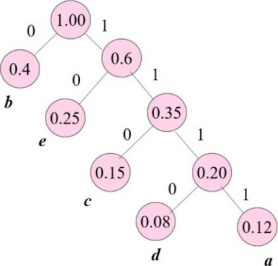
\includegraphics[width=0.4\textwidth]{images/exp5-1.png}
\hspace{1em}
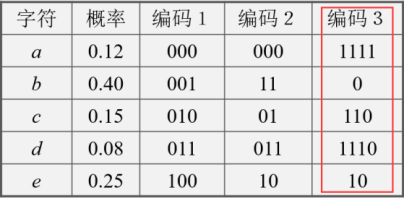
\includegraphics[width=0.5\textwidth]{images/exp5-2.png}
\end{center}
\begin{center}
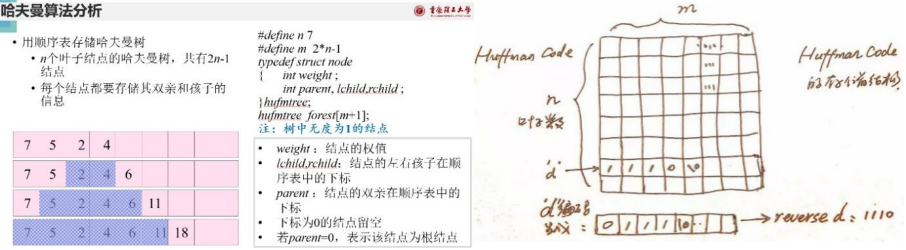
\includegraphics[width=0.95\textwidth]{images/exp5-3.png}
\end{center}
\noindent\hspace*{2em}给定文件文件：huffmandata.txt\par
\noindent\hspace*{2em}\textbf{输}\textbf{文件：}\textbf{huffmandata.zipe}\par
\sect{实验结果}
\noindent\hspace*{2em}1. 算法概述：简述算法框架\par
\noindent\hspace*{2em}2. 实验重点或难点\par
\noindent\hspace*{2em}（1）\par
\noindent\hspace*{2em}（2）\par
\noindent\hspace*{2em}3. 实验结果\par
\noindent\hspace*{2em}（1）实验测试描述，及运行结果记录\par
\noindent\hspace*{2em}4. 实验方案分析\par
\noindent\hspace*{2em}（1）本实验设计的优点，不足，时空开销等问题分析\par
\noindent\hspace*{2em}5. 附件：源程序代码\par
\noindent\hspace*{2em}源代码复制粘贴在这里（六号字，分栏，单倍行距不要对齐网格）\par
\clearpage
\expchapter{实验六\quad 谁是网络大 V?}
\sect{教学目标}
\noindent\hspace*{2em}关键词：图\par
\noindent\hspace*{2em}知识和能力目标：理解和熟练掌握图的存储及操作方法，本例主要是计算有向图中顶点的度，并做进一步的应用。\par
\noindent\hspace*{2em}价值目标：\par
\noindent\hspace*{2em}科学精神：一个问题、一个方案的评价指标往往不是唯一的，也常常没有标准答案。为了找到网络大V，其相关指标众多，需要研究者根据具体问题进行分析、确定和实验验证。\par
\noindent\textbf{工程与社会：}\par
\noindent\textbf{你知道新浪微博红V、蓝 V、金 V 的区别吗？}\par
\noindent\hspace*{2em}你认为网络大V 可能对社会，尤其是社交网络中的青少年群体起到什么样的作用？你是否曾受到过网络大V 的影响？\par
\sect{问题描述}
\noindent\hspace*{2em}社交网络可抽象为一种图结构。进一步地，从社交网络用户的关注、被关注关系角度观察，可将这种图看成是有向图。例如，如果一个用户 \textit{u}\textit{ }被 100 个粉丝关注，不妨认为 \textit{u}\textit{ }的入度为 100，如果 \textit{u }关注了 1000 个账号，则 \textit{u }的出度为 1000。\par
\begin{center}
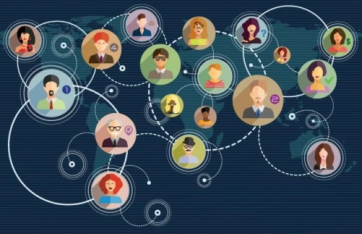
\includegraphics[width=0.4\textwidth]{images/exp6-1.png}
\hspace{1em}
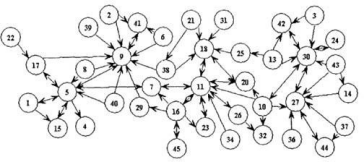
\includegraphics[width=0.5\textwidth]{images/exp6-2.png}
\end{center}
\noindent\hspace*{2em}大 V\footnote{源自百度百科词条：网络大 V}一般指在微博上十分活跃、有着大群粉丝的用户。“V”（Verified）指用户已通过认证，经微博身份认证的账户名后会显示 V 字符。大V 拥有百万计甚至千万计的粉丝，可能成为微博“意见领袖”，带动微博用户活跃度。如果大 V 把未经核实的谣言随意转载引用，则将推动谣言快速传播。\par
\begin{center}

\includegraphics[width=0.75\textwidth]{images/exp6-3.png}
\end{center}
\noindent\hspace*{2em}社会网络\footnote{最初对社会网络感兴趣的是英国著名的人类学家布朗(Radcliffe Brown)。他在对社会结构的关注中，以相对非技术的形式提出了“社会网络”（Social Network）的思想。}（social network）分析中有一个度中心性（\textbf{Degree}\textbf{ }\textbf{Centrality}）指标，是刻画结点中心性（Centrality）的直接度量指标之一：\par
\noindent\hspace*{2em}度中心性\footnote{社交网络分析中重要指标：\url{https://blog.csdn.net/weixin_43841231/article/details/100114506}}：一个结点的度越大，意味着该结点的度中心性越高，其在网络中就越重要。例如，用户 \textit{u}1 有 20 个微信好友，\textit{u}2 有 50 个好友，则 \textit{u}1 的度中心性大于 \textit{u}2，其社交圈子可能更广。显然，本例是无向图的情形，如果是有向图，则需考虑出度和入度问题。\par
\noindent\hspace*{2em}【拓展问题】如何比较用户 \textit{\textbf{u}}\textit{\textbf{ }}在微博和微信上的度中心性？如果微信与微博的人数规模相当，则可以直接比较，但如用户数存在规模差异，则需考虑去规模化问题，即标准化度中心性。\par
\noindent\textbf{本实验要求：}\par
\noindent\hspace*{2em}对一个给定的社交网络图，找出其中大 \textbf{V}\textbf{ }结点。\par
\sect{基本思路}
\noindent\textbf{基本假设：}\par
\noindent\hspace*{2em}不妨以度中心性为指标，确定网络大 V：考虑社会网络是微博（故为有向图），度中心性指计算结点的入度。\par
\noindent\hspace*{2em}如果某结点的入度在网络中排名前 10，则该结点是大V 结点。\par
\noindent\hspace*{2em}对输出形式无特殊要求，输出大V 结点的 ID 即可。\par
\noindent\hspace*{2em}数据来源：http://www.sociopatterns.org/datasets/\par
\noindent\hspace*{2em}The data set gives the contacts of the students of nine classes during 5 days in Dec. 2013\par
\noindent\hspace*{2em}不妨用邻接矩阵来存储图。由于是有向图，因此矩阵非对称。\par
\sect{实验结果}
\noindent\hspace*{2em}1. 算法概述：简述算法框架\par
\noindent\hspace*{2em}2. 实验重点或难点\par
\noindent\hspace*{2em}（1）\par
\noindent\hspace*{2em}（2）\par
\noindent\hspace*{2em}3. 实验结果\par
\noindent\hspace*{2em}（1）实验测试描述，及运行结果记录\par
\noindent\hspace*{2em}4. 实验方案分析\par
\noindent\hspace*{2em}（1）本实验设计的优点，不足，时空开销等问题分析\par
\noindent\hspace*{2em}5. 附件：源程序代码\par
\noindent\hspace*{2em}源代码复制粘贴在这里（六号字，分栏，单倍行距不要对齐网格）\par
\clearpage
\expchapter{实验七\quad 我的搜索引擎 MARS}
\sect{教学目标}
\noindent\hspace*{2em}关键词：搜索引擎，倒排索引\par
\noindent\hspace*{2em}知识和能力目标：理解和熟练掌握多链表存储结构及操作方法，本例主要是构建倒排索引结构，进而构建一个简易的搜索引擎。\par
\noindent\hspace*{2em}价值目标：科学精神：信息检索系统中包含的原理、方法和实践技术庞大，本实验仅仅只窥一斑。希望你能立足本实验，从查询分析、索引建立、结果排序等各方面，做进一步的探索。要相信，知之越多，知之越少，探究得更深入，才能越知自己的不足。\par
\sect{问题描述}
\noindent\hspace*{2em}搜索引擎是指从互联网上采集、组织和处理信息，进而提供信息检索服务、将检索结果展示给用户的系统。搜索引擎旨在提供快速、高相关性的信息服务，搭建起友好的网络使用平台。搜索引擎涵盖信息存储、检索等多种技术，如网络爬虫、检索排序、网页处理、自然语言处理等，因此其核心模块一般包括爬虫、索引、检索和排序等\footnote{同时可添加其他辅助模块，为用户提供更好的信息检索体验。}。图 1 是一个信息检索过程的简图。\par

\noindent\textbf{\textbf{Result}}\par
\begin{center}
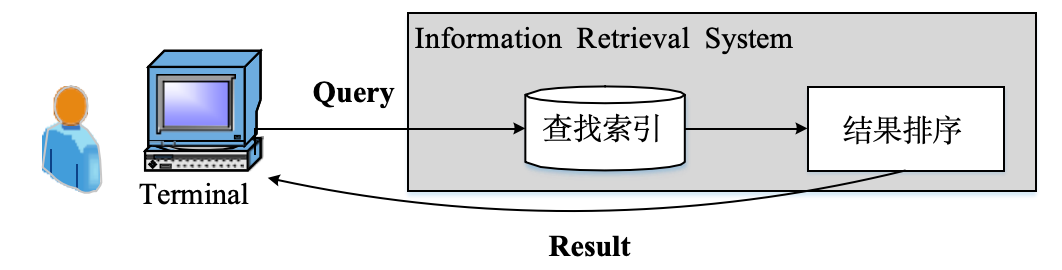
\includegraphics[width=0.7\textwidth]{images/exp7-1.png}
\end{center}
\figcaption{图 1 信息检索过程简图}
\noindent\hspace*{2em}现在我们聚焦图 1 的“查找索引”环节。显然，为了查找，需构建一个“查找表”，也可叫它 “索引库”。根据用户提交的搜索请求（Query），去查找表中找到相关文档或网页，再通过对网页进行重要性排序等操作，把查询结果反馈给用户。\par
\noindent\hspace*{2em}在构建查找表时，其策略是构造“文档—词项关联矩阵”（图 2（a））或“词项—文档关联矩阵”（图 2（b））所示。它们的检索效率会有什么不同呢？\par
\begin{center}
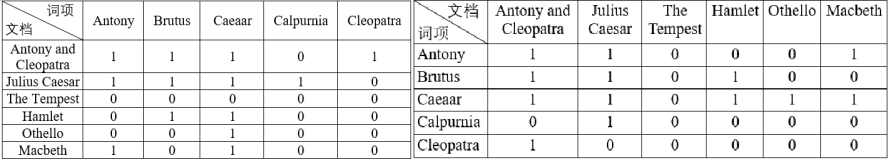
\includegraphics[width=0.95\textwidth]{images/exp7-3.png}
\end{center}
\figcaption{图 2 两种查找表构建策略}
\noindent\hspace*{2em}为保证存储和查找效率，常以如下倒排索引（Inversed Index）的（图 3）方法构造查找表。\par
\begin{center}
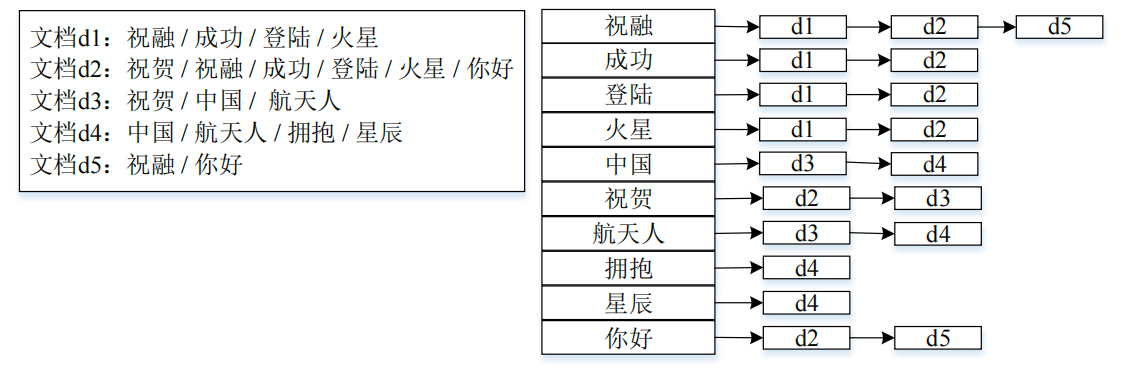
\includegraphics[width=0.7\textwidth]{images/exp7-2.png}
\end{center}
\figcaption{图 3 倒排索引结构示例}
\noindent\textbf{本实验要求：}\par
\noindent\hspace*{2em}构建一个我们自己的搜索引擎。很高兴，2022 年 5 月 15 日，中国的“天问一号”搭载火星车“祝融”成功登陆火星，拓展了中国人逐梦星辰的疆域。我们把我们的搜索引擎起名为小马尔斯（\textbf{M}\textbf{A}\textbf{R}\textbf{S}），以庆祝这个重要的时刻。\par
\noindent\hspace*{2em}MARS 的主要任务：用户可输入一个关键词，MARS 到查找表中去找到这个关键词相关的文本，返回这些文本。\par
\sect{基本思路}
\noindent\textbf{基本假设：}\par
\noindent\hspace*{2em}用户每次只输入一个关键词，例如：apple\par
\noindent\hspace*{2em}MARS 只需返回所有与关键词相关的文本文件名，无需对这些文本进行排序。\par
\noindent\hspace*{2em}对输出格式无要求，MARS 只需显示相关文本的文件名即可。以下为一种运行情境示例。在控制台输入snow，将检索结果输出到 index.html 文件，可在浏览器中打开 index.html 文件进行浏览。\par
\begin{center}
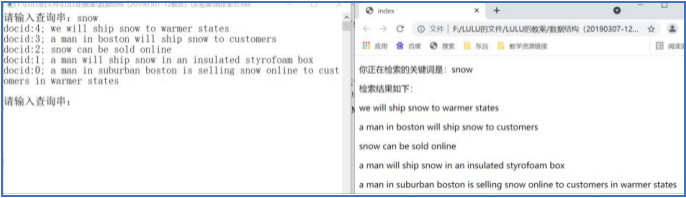
\includegraphics[width=0.95\textwidth]{images/exp7-4.png}
\end{center}

\sect{实验结果}
\noindent\hspace*{2em}1. 算法概述：简述算法框架\par
\noindent\hspace*{2em}2. 实验重点或难点\par
\noindent\hspace*{2em}（1）\par
\noindent\hspace*{2em}（2）\par
\noindent\hspace*{2em}3. 实验结果\par
\noindent\hspace*{2em}（1）实验测试描述，及运行结果记录\par
\noindent\hspace*{2em}4. 实验方案分析\par
\noindent\hspace*{2em}（1）本实验设计的优点，不足，时空开销等问题分析\par
\noindent\hspace*{2em}5. 附件：源程序代码\par
\noindent\hspace*{2em}源代码复制粘贴在这里（六号字，分栏，单倍行距不要对齐网格）\par
\clearpage
\expchapter{实验八\quad 组织小型家庭宴会}
\sect{教学目标}
\noindent\hspace*{2em}关键词：图，关键路径\par
\noindent\hspace*{2em}知识和能力目标：理解关键路径的基本概念，理解查找图中关键路径的算法原理，能够根据问题构建图存储结构，并找出其中的关键路径。\par
\noindent\hspace*{2em}价值目标：\par
\noindent\hspace*{2em}(1) 人文素质：\par
\sect{问题描述}
\noindent\hspace*{2em}关键路径（Critical Path）是指设计中从输入到输出经过的延时最长的逻辑路径。在项目计划中，关键路径通常是决定项目工期的进度活动序列，它是项目中最长的路径，即使很小的浮动，也可能直接影响整个项目的最完成时间，因此，优化关键路径是一种优化项目工期的有效方法。\par
\begin{center}
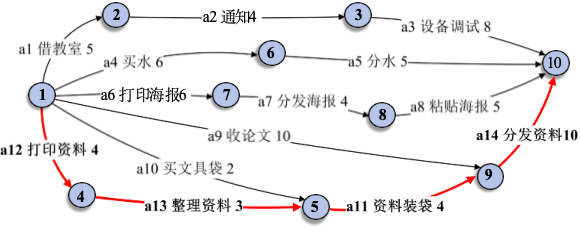
\includegraphics[width=0.7\textwidth]{images/exp8-1.png}
\end{center}
\figcaption{图 1 毕业设计答辩筹备工作计划图}
\noindent\hspace*{2em}在分析项目的进度计划时，我们通常可以用顶点表示事件，弧表示活动，弧上的权值表示活动持续的时间，由此将项目进度计划抽象为一幅有向图，也称AOE（Activity On Edge Network）网。 AOE 网常用于估算项目完成时间。例如，图 1 是根据毕业设计答辩筹备工作计划绘制的 AOE 网。其中，有 10 个事件 1,2,…,10；14 项活动 a1,a2,…,a14。每个事件表示在它之前的活动已经完成，在它之后的活动可以开始。其中，事件 1 为整个计划的开始（也称源点），事件 10 表示整个计划结束\par
\noindent （也称汇点）。事件 5 表示活动 a10 和 a13 已经完成，活动 a11 可以开始。弧上的权表示完成该活动所需的时间。如活动 a1 需要 5 个时间单位完成。\par
\noindent\hspace*{2em}在图 1 中，活动a12 a13 a11 a14 是一条长度为 21 的关键路径，它是毕业设计答辩筹备所需要的最长时间。要注意的是，一个项目中可能有多个、并行的关键路径。\par
\noindent\hspace*{2em}关键路径方法是由杜邦公司\footnote{关键路径法（CPM）最出现于 1956 年，当时美国杜邦（Du Pont）公司的主要负责人 Morgan Walker 和雷明顿兰德（Remington Rand）公司的数学家 James E. Kelly 研究如何能够采取正确的措施，在减少工期的情况下能尽可能少地增加费用。（\url{https://baike.baidu.com/item/关键路径法}）}发明的。\par
\noindent\hspace*{2em}我们通过以下项目的例子\footnote{https://wenku.baidu.com/view/b896d8acad1ffc4ffe4733687e21af45b207fe27.html}来说明如果找到关键路径。该项目是对某公司的办公室重新进行装修，拆掉办公室里面的非承重墙，改造原来的谁、电、气线路，装上智能楼宇控制系统，并更换部分办公家具，请确定项目的关键路径。项目各活动的时间如图 2(a)所示，我们按照图 2(b)所示形式来描述各活动结点，各活动的前后关系如图 3 所示，寻找关键路径的过程如图 4\textasciitilde{}图 7 所示。\par
\begin{center}
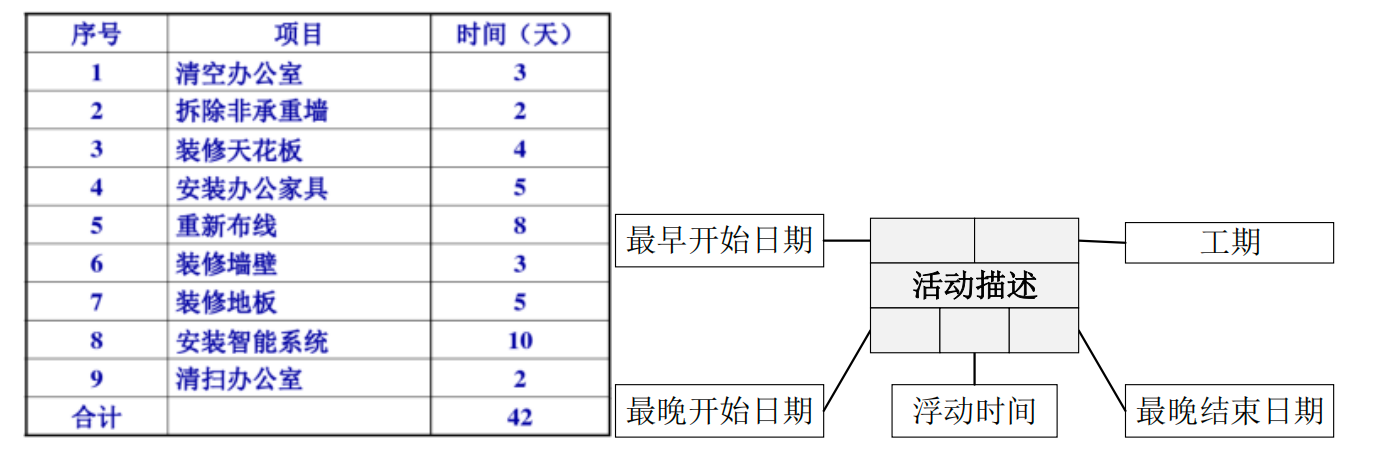
\includegraphics[width=0.95\textwidth]{images/exp8-2.png}
\end{center}
\figcaption{图 2 项目活动时间表及活动结点结构}
\begin{center}
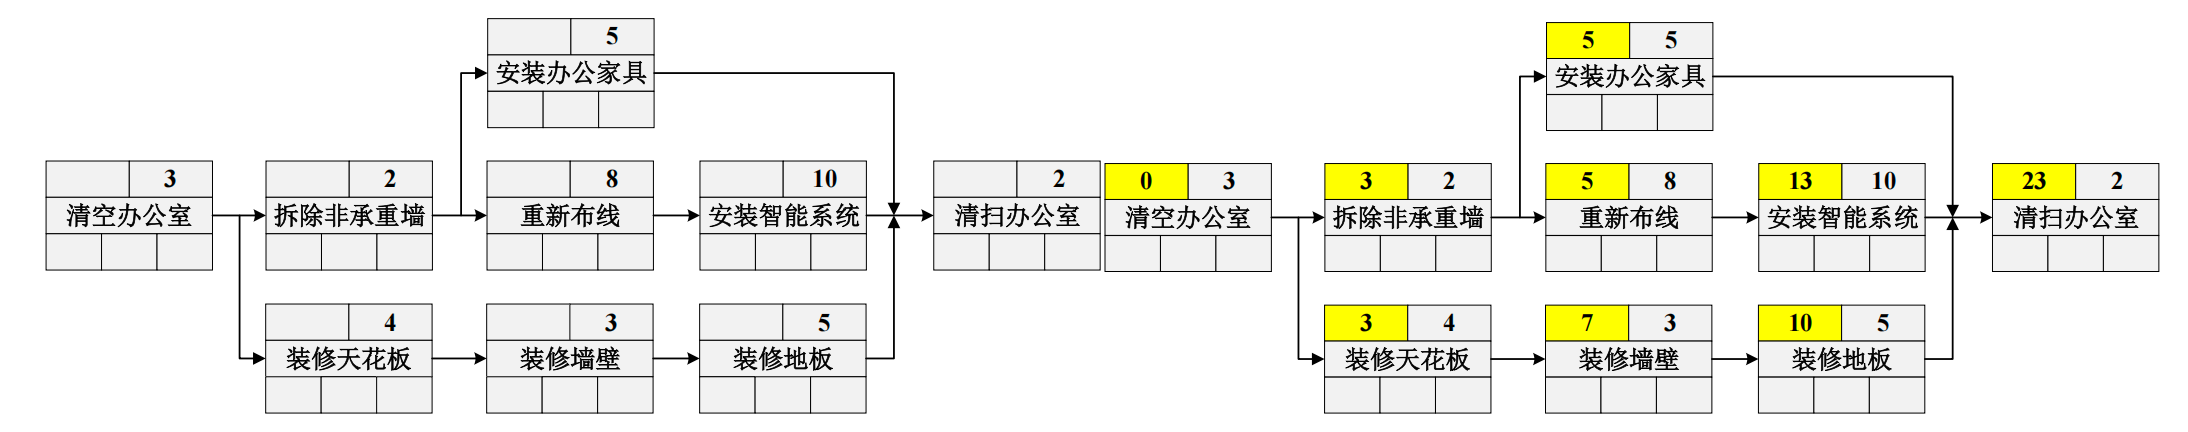
\includegraphics[width=0.95\textwidth]{images/exp8-3.png}
\end{center}
\begin{minipage}{0.48\textwidth}
\centering\figcaption{图 3 工作计划图前后关系及初始状态}
\end{minipage}\hfill
\begin{minipage}{0.48\textwidth}
\centering\figcaption{图 4 填写各活动的最开始时间}
\end{minipage}
\begin{center}
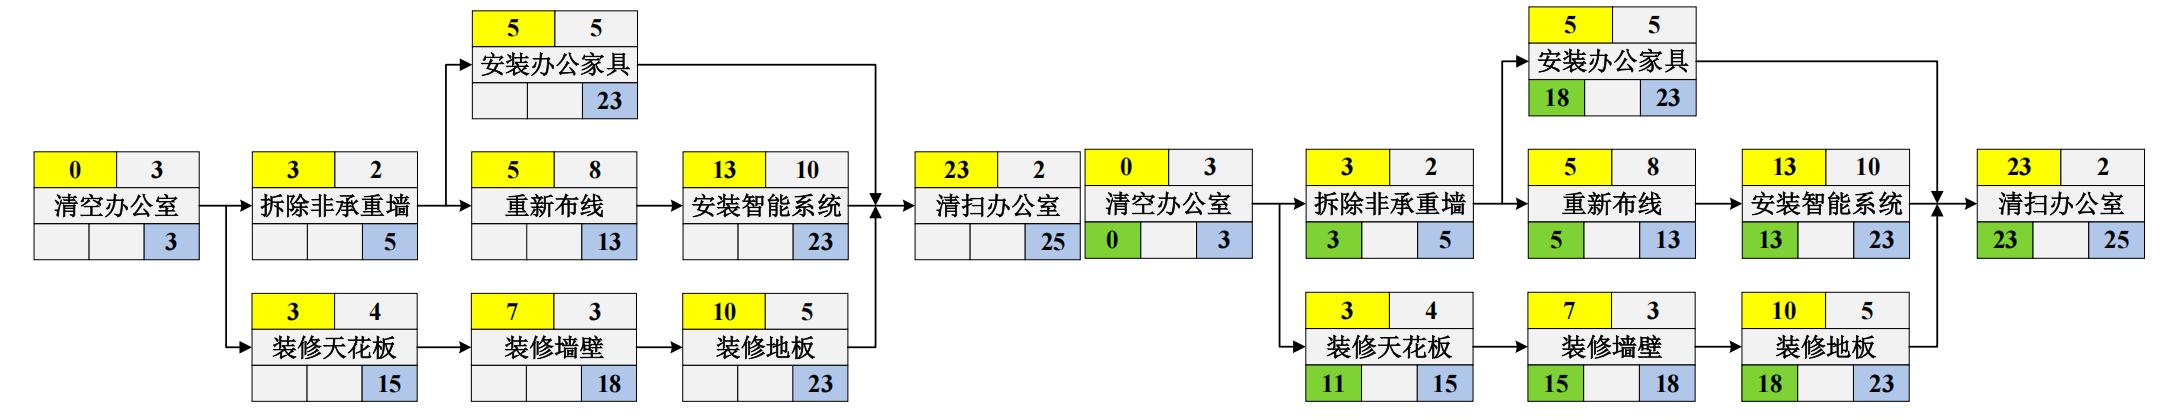
\includegraphics[width=0.95\textwidth]{images/exp8-4.png}
\end{center}
\begin{minipage}{0.48\textwidth}
\centering\figcaption{图 5 填写各活动的最晚结束时间}
\end{minipage}\hfill
\begin{minipage}{0.48\textwidth}
\centering\figcaption{图 6 填写各活动的最晚开始时间}
\end{minipage}
\begin{center}
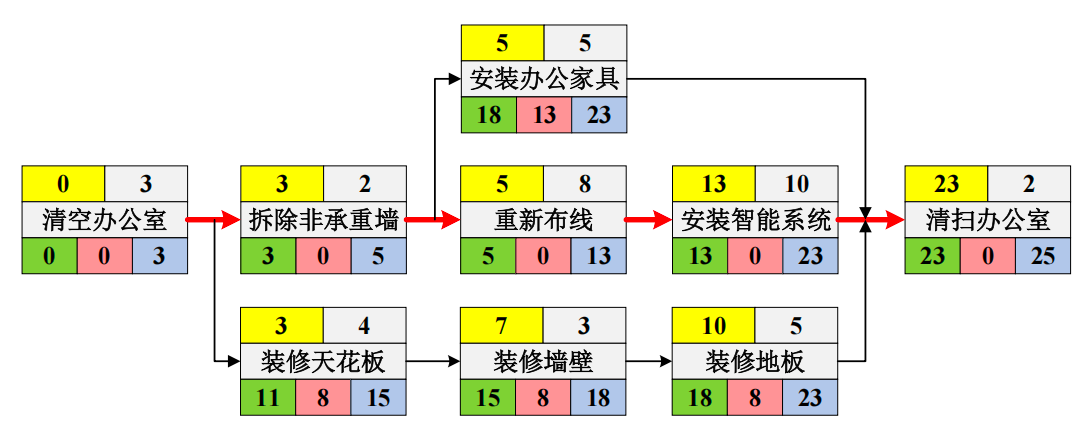
\includegraphics[width=0.95\textwidth]{images/exp8-5.png}
\end{center}
\figcaption{图 7 填写各活动的浮动时间}
\begin{center}
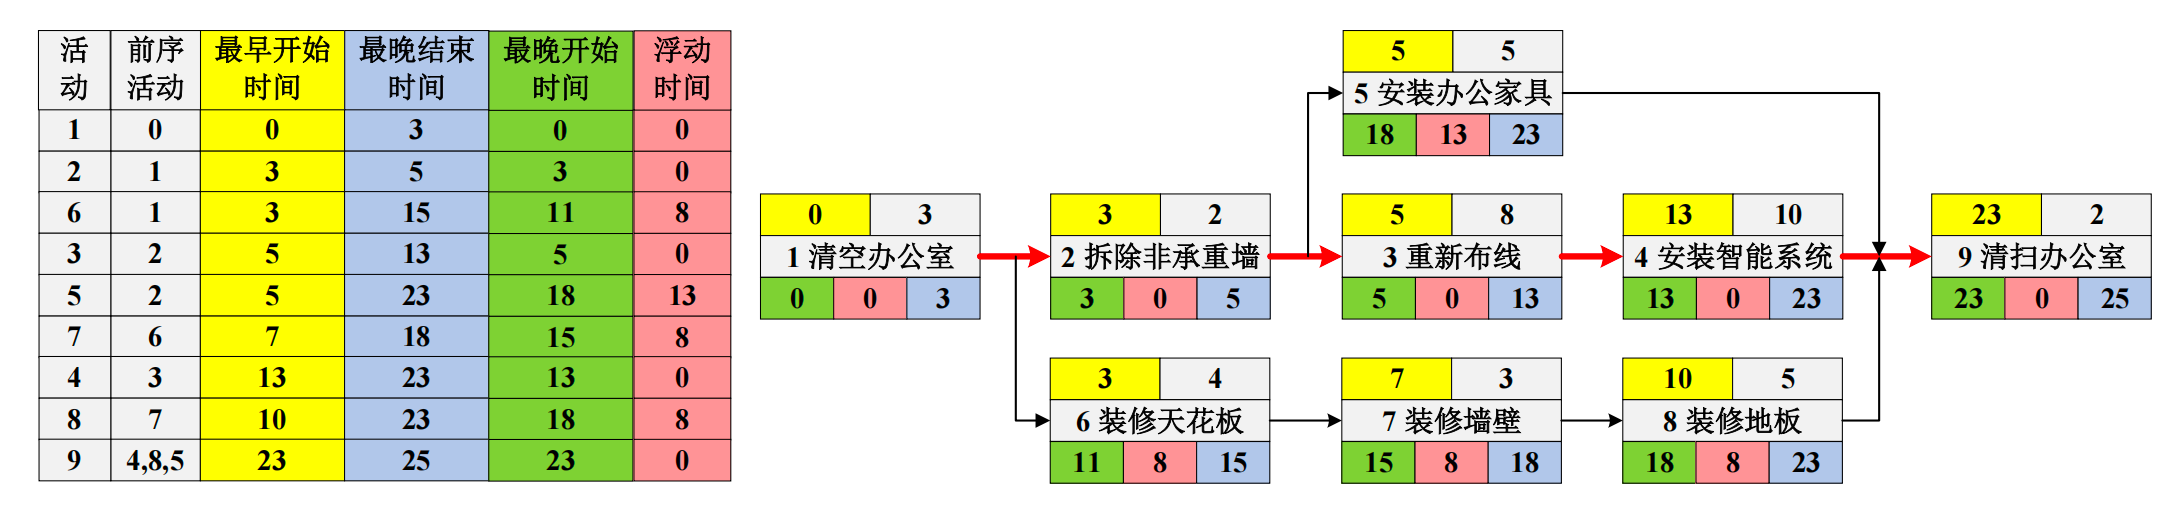
\includegraphics[width=0.95\textwidth]{images/exp8-6.png}
\end{center}
\figcaption{图 8 依据事件（顶点）的拓扑序列计算各项时间}
\noindent\hspace*{2em}本问题的任务是：\par
\noindent\hspace*{2em}编写程序，筹备一个小型家庭宴会，做多需要多少准备时间？假设如下：\par
\noindent\hspace*{2em}假设宴会筹备\footnote{https://wenku.baidu.com/view/b896d8acad1ffc4ffe4733687e21af45b207fe27.html}的各活动如图 9(a)所示，因此筹备进度的初始状态图如图 9(b)所示。\par
\noindent\hspace*{2em}输出形式不限。\par

\sect{基本思路}
\noindent\hspace*{2em}根据宴会活动构建图。\par
\noindent\hspace*{2em}查找关键路径，填充左下表（填充结果如下右图所示）：\par
\noindent\textbf{对图进行拓扑排序，填充第 1、2 列}\par
\noindent\hspace*{2em}按照拓扑排序的顶点顺序，正向填充黄色列\par
\noindent\textbf{按照拓扑排序的顶点顺序，逆向填充蓝色列}\par
\noindent\textbf{按照拓扑排序的顶点顺序，正向填充绿色列}\par
\noindent\textbf{填充粉色列}\par
\noindent\hspace*{2em}关键问题：\par
\noindent\textbf{定义合理的图存储结构，以及上表的存储结构}\par
\noindent\textbf{为便于拓扑排序和访问，可考虑采用图的十字链表存储}\par
\sect{实验结果}
\noindent\hspace*{2em}1. 算法概述：简述算法框架\par
\noindent\hspace*{2em}2. 实验重点或难点：\par
\noindent\hspace*{2em}3. 实验结果：实验测试描述，及运行结果记录\par
\noindent\hspace*{2em}4. 实验方案分析：本实验设计的优点，不足，时空开销等问题分析\par
\noindent\hspace*{2em}5. 附件：源程序代码：源代码复制粘贴在这里（六号字，分栏，单倍行距不要对齐网格）\par
\end{document}
